\section{Vorlesung 15.06.2016}

\subsection{Gal4 / UAS-System: MARCM}
 - \textbf{M}osaic \textbf{a}nalysis with a \textbf{r}epressible \textbf{c}ell \textbf{m}arker\footnote{\url{https://en.wikipedia.org/wiki/MARCM}}\\

\underline{es werden 5 Transgene (eingeschleuste Gene) benötigt:}
\begin{itemize}
	\item Gal4/ UAS pair
	\item Gal80
	\item Flp/FRT-System\footnote{\url{https://de.wikipedia.org/wiki/Flp/FRT-System}}: zur Entfernung oder Einfügung von DNA-Sequenzen (Heatshock)
		\begin{itemize}
			\item FLP-Rekombinase (Flippase) um DNA-Sequenzen ortsspezifisch auszutauschen
			\item FRT (FLP recognition target) DNA Sequenz
		\end{itemize}
\end{itemize}

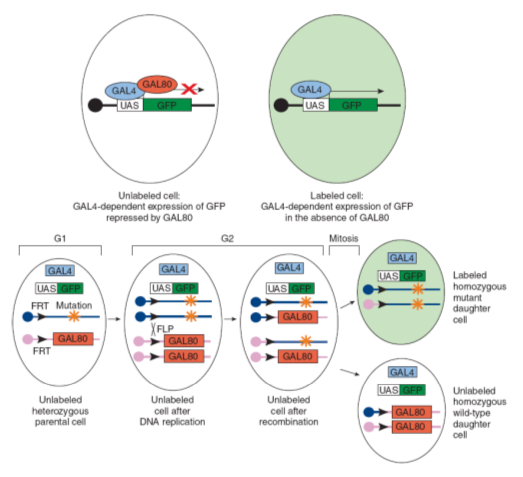
\includegraphics[width=0.9\textwidth]{lectures/160615/pix/marcm.png}

\subsection{Gedächtnisbildung: Phasen in Drosophila}
\begin{enumerate}
	\item acquisition: Aneignung
	\item short-term memory (STM)
	\item middle-term memory (MTM)
	\item anesthesia-resistant memory (ARM)
	\item long-term memory (LTM)
\end{enumerate}

\underline{Versuch zum Kurzzeitgedächtnis bei Drosophila:}\\
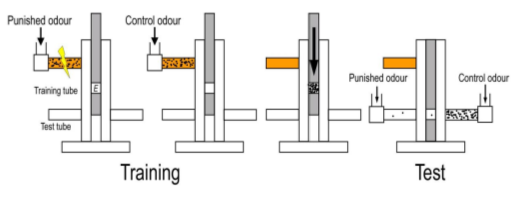
\includegraphics[width=0.6\textwidth]{lectures/160615/pix/short_term_memory_drsophila.png}

\subsection{Klassisches Konditionieren}
 - Diese Mechanismen scheinen in allen Tierarten von der Schnecke bis zum Menschen prinzipiell sehr ähnlich abzulaufen (evolutionär konserviert)

\textbf{J.B. Watson's Experiment am kleinen Albert}
\begin{itemize}
	\item Experiment zur klassischen Konditionierung am Menschen
	\item natürliches Interesse an Objekten wie Kaninchen, Affe, Ratte
	\item dann Konditionierung: die gleichen Objekten wurden wieder gezeigt, jedoch verbunden mit lautem Geräusch (Schlag mit Hammer auf Eisenstange)
	\item nach Konditionierung: Angst vor den gleichen Objekten
\end{itemize}

\subsection{olfaktorisches Lernen bei Drosophila}
\textcolor{red}{\textbf{!!!muss noch gemacht werden!!!}}

\textbf{Role of Synaptic Vesicle Proteins}
